\documentclass[aspectratio=169]{beamer}
\usepackage{color,amsmath}
\usepackage{subfigure}
\usepackage{booktabs}
\usepackage{framed}
\usepackage{comment}

\def\vf{\vfill}

%%%%%%%%%%%%%%%%%%%%%%%%%%
\title[]{Forecasting and Google Flu Trends (02-05)}
\author[]{Matthew J. Salganik\\Department of Sociology\\Princeton University}
\date[]{Soc 596: Computational Social Science
\vfill
\begin{flushright}
\vspace{0.6in}

\includegraphics[width=0.1\textwidth]{figures/cc.png}
\end{flushright}
}
\begin{document}
%%%%%%%%%%%%%%%%%%%%%%%%%%
\frame{\titlepage}
%%%%%%%%%%%%%%%%%%%%%%%%%%
\begin{frame}

\begin{center}
prediction vs forecasting
\end{center}

\end{frame}
%%%%%%%%%%%%%%%%%%%%%%%%%%
\begin{frame}

\begin{center}
Rain dance problems vs umbrella problems (Kleinberg et al 2015)
\end{center}

\end{frame}
%%%%%%%%%%%%%%%%%%%%%%%%%%
\begin{frame}

\begin{center}
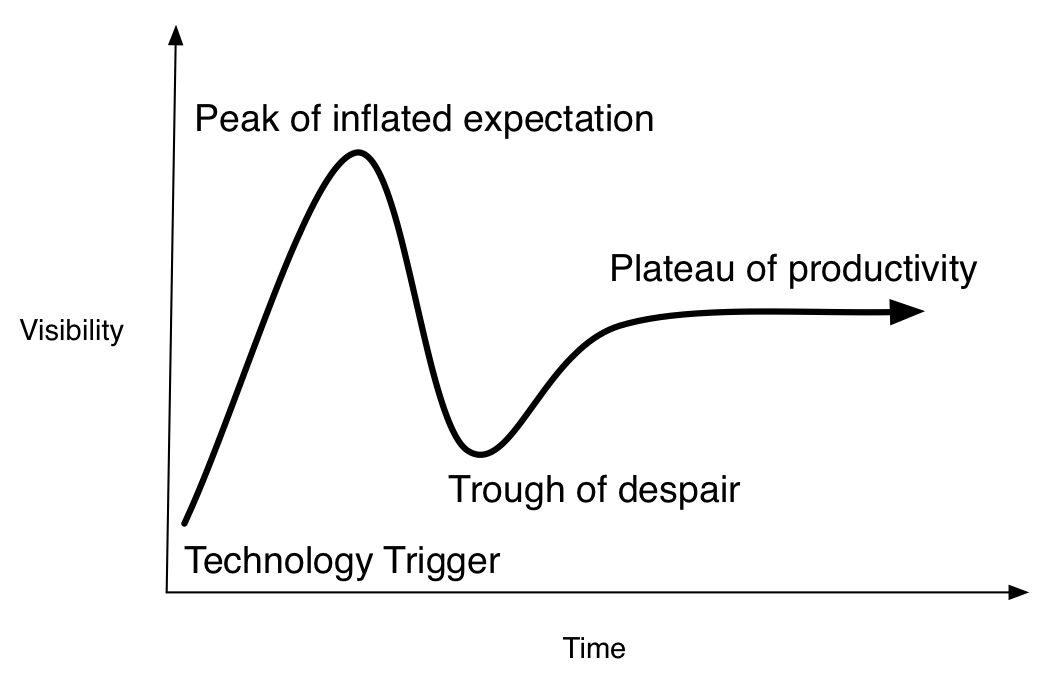
\includegraphics[width=\textwidth]{figures/hype_cycle}
\end{center}

\vf
\tiny{Fenn and Raskino (2008)}

\end{frame}
%%%%%%%%%%%%%%%%%%%%%%%%%%
\begin{frame}

Watch the progression . . . . .

\end{frame}
%%%%%%%%%%%%%%%%%%%%%%%%%%
\begin{frame}

\begin{center}
\includegraphics[width=\textwidth]{figures/eysenbach_infodemiology_2006_title}
\end{center}

\vf
Eysenbach (2006) ``Infodemiology: Tracking Flu-Related Searches on the Web for Syndromic Surveillance'', American Medical Informatics Association
Annual Symposium Proceedings, \url{http://www.ncbi.nlm.nih.gov/pmc/articles/PMC1839505/}

\end{frame}
%%%%%%%%%%%%%%%%%%%%%%%%%%
\begin{frame}

\begin{center}
\only<1>{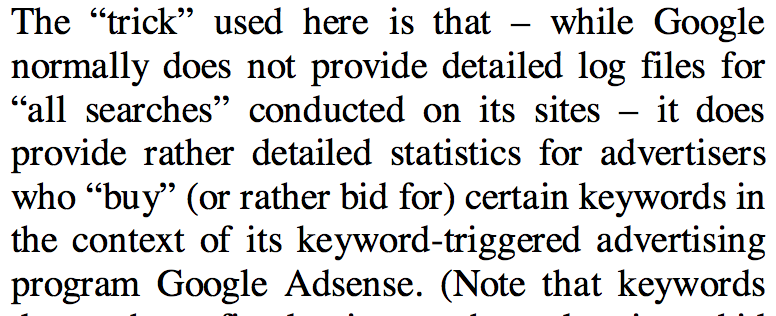
\includegraphics[width=\textwidth]{figures/eysenbach_infodemiology_2006_trick}}
\only<2>{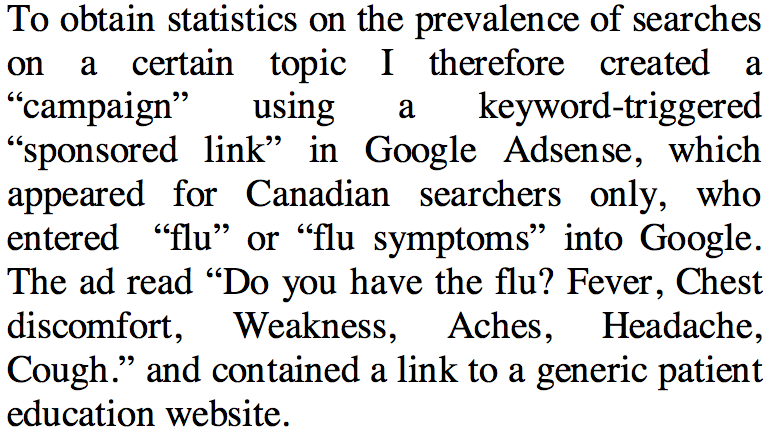
\includegraphics[width=\textwidth]{figures/eysenbach_infodemiology_2006_ad}}
\only<3>{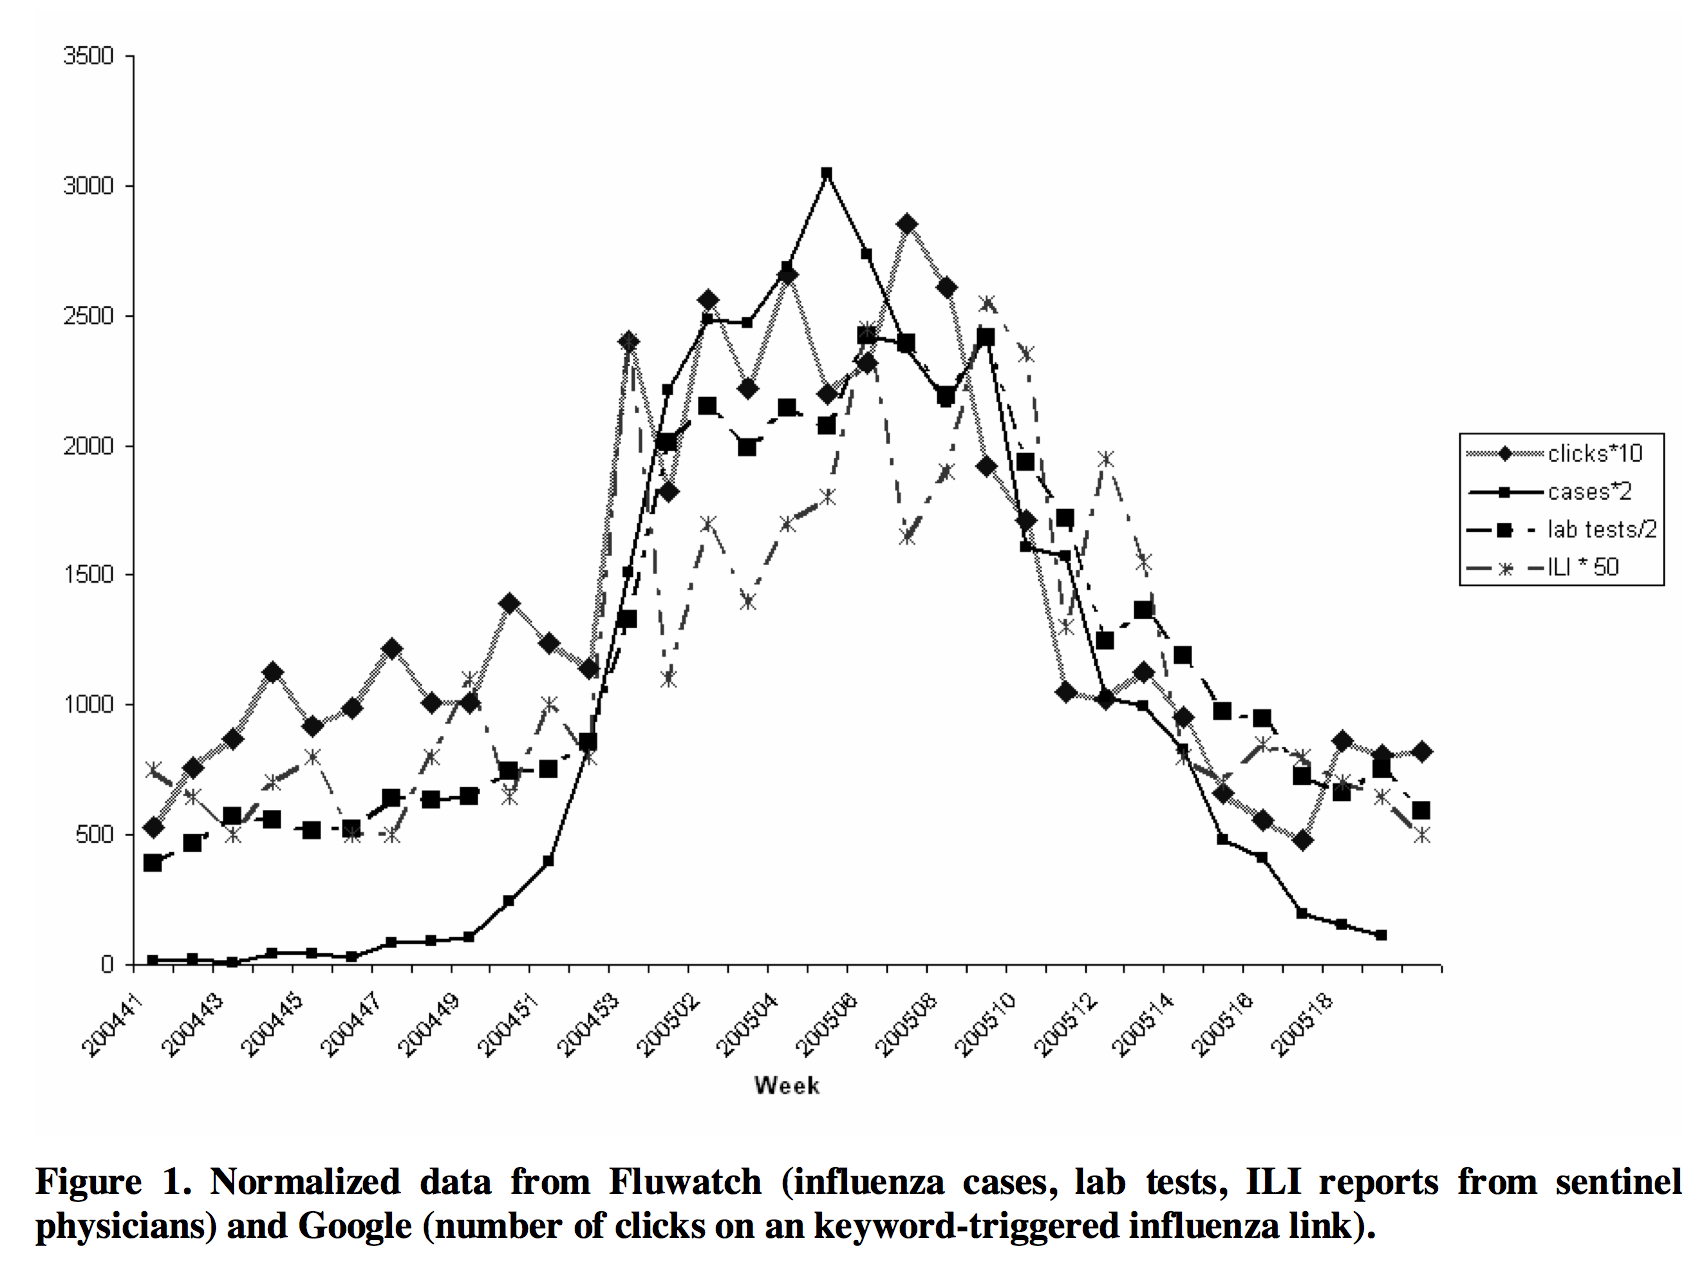
\includegraphics[width=\textwidth]{figures/eysenbach_infodemiology_2006_fig1}}
\end{center}

\end{frame}
%%%%%%%%%%%%%%%%%%%%%%%%%%
\begin{frame}

{\Large
\begin{center}
Aside: Interesting use of ad-click rates.
\end{center}
}

\end{frame}
%%%%%%%%%%%%%%%%%%%%%%%%%%
\begin{frame}

\begin{center}

\includegraphics[width=\textwidth]{figures/polgreen_using_2008_title}
\end{center}

\vf
Polgreen et al. (2008) ``Using Internet Searches for Influenza Surveillance'', \textit{Clinical Infectious Diseases}, \url{http://dx.doi.org/10.1086/593098}

\end{frame}
%%%%%%%%%%%%%%%%%%%%%%%%%%
\begin{frame}

\begin{center}
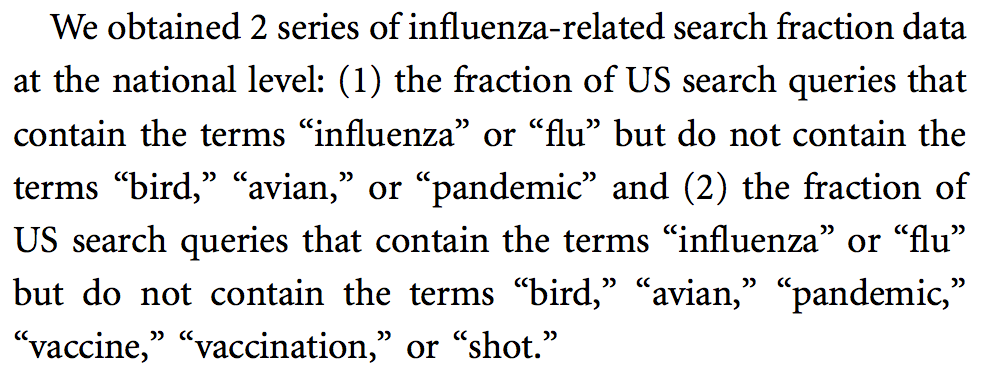
\includegraphics[width=\textwidth]{figures/polgreen_using_2008_data}
\end{center}

\vf
Note that they had access to raw search data from Yahoo!

\end{frame}
%%%%%%%%%%%%%%%%%%%%%%%%%%
\begin{frame}

\begin{center}
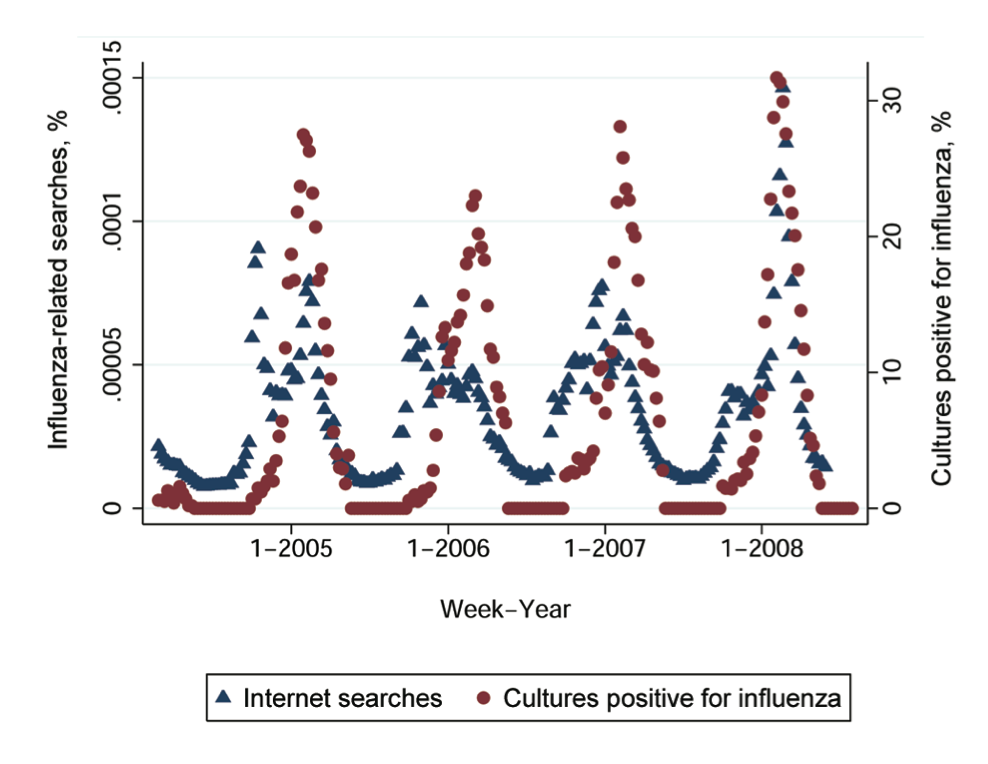
\includegraphics[width=\textwidth]{figures/polgreen_using_2008_fig1}
\end{center}

\end{frame}
%%%%%%%%%%%%%%%%%%%%%%%%%%
\begin{frame}

\begin{center}
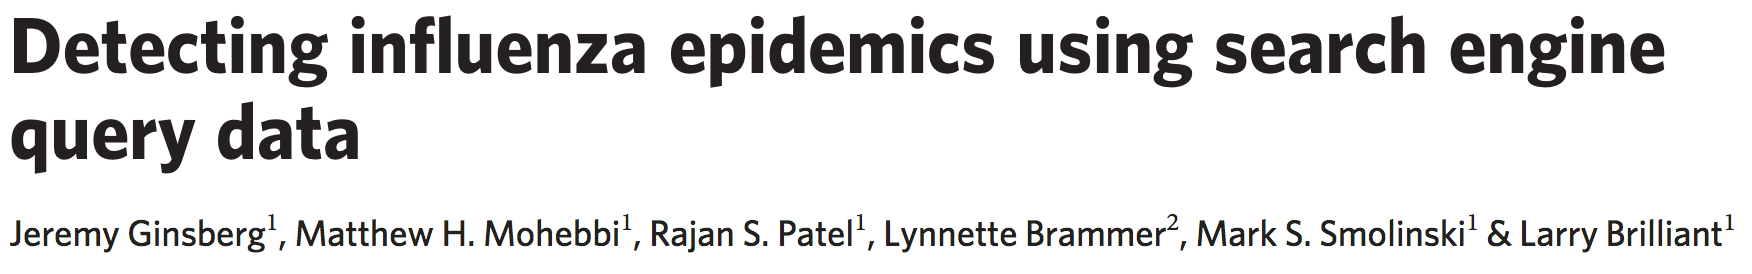
\includegraphics[width=\textwidth]{figures/ginsberg_detecting_2009_title}
\end{center}

\vf
Ginsberg et al. (2009) ``Detecting influenza epidemics using search engine query data'', \textit{Nature}, \url{http://dx.doi.org/10.1038/nature07634}

\end{frame}
%%%%%%%%%%%%%%%%%%%%%%%%%%
\begin{frame}

\begin{center}
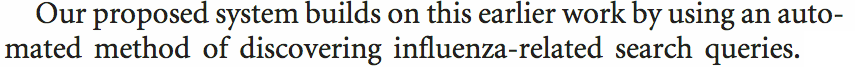
\includegraphics[width=\textwidth]{figures/ginsberg_detecting_2009_data}
\end{center}

\end{frame}
%%%%%%%%%%%%%%%%%%%%%%%%%
\begin{frame}

Key idea from data science:\\
Over-fitting

\end{frame}
%%%%%%%%%%%%%%%%%%%%%%%%%
\begin{frame}

\begin{center}
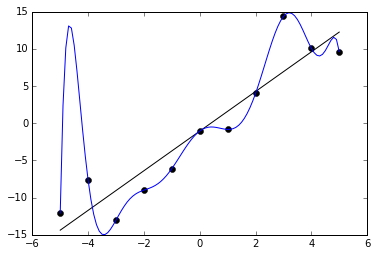
\includegraphics[width=0.8\textwidth]{figures/overfitted_data}
\end{center}

\textcolor{green}{Which line fits the data better?}
\begin{enumerate}
\item straight line
\item curved line
\end{enumerate}

\vf
\TINY{\url{https://commons.wikimedia.org/wiki/File:Overfitted_Data.png}}

\end{frame}
%%%%%%%%%%%%%%%%%%%%%%%%%
\begin{frame}

Keyword selection method:
\begin{itemize}
\item Try 50 million keywords and see which ones work best
\end{itemize}

\end{frame}
%%%%%%%%%%%%%%%%%%%%%%%%%
\begin{frame}

Keyword selection method (roughly):
\begin{itemize}
\item For each possible keyword
\item For each region
\item Split 128 outcome measures (CDC flu measurements) into 4 sets of 96 outcome measures 
\item Fit linear regression: $I(t) = \beta_0 + \beta_1 Q(t)$
\item Use fitted weights to predict held out 32 values (96 + 32 = 128) 
\item Calculate correlation between predicted values and actual values
\item Average (transformed) correlations across cross validations and regions
\end{itemize}
\vf
Then, find sets of keywords that work well together
\end{frame}
%%%%%%%%%%%%%%%%%%%%%%%%%
\begin{frame}

\begin{center}
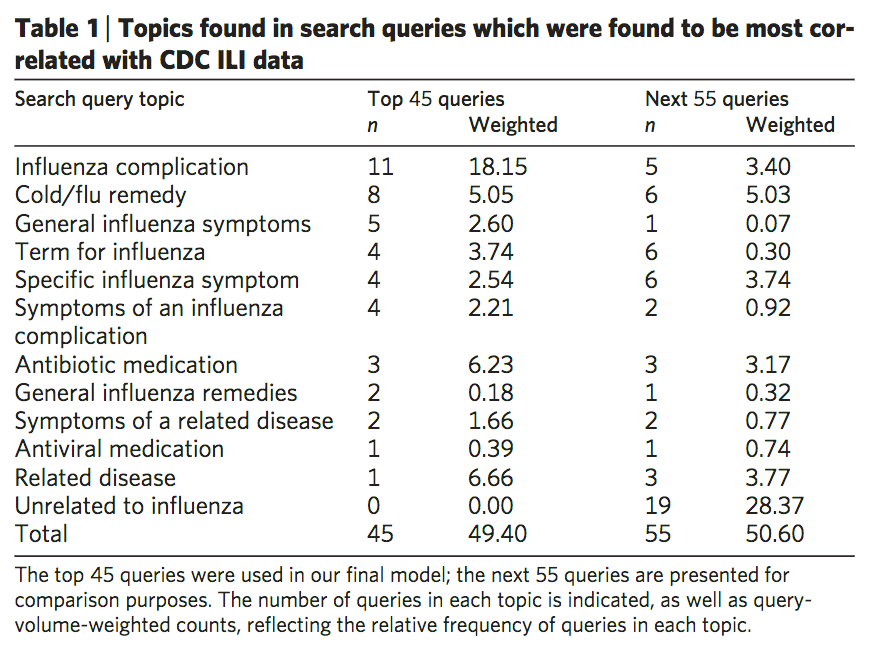
\includegraphics[width=\textwidth]{figures/ginsberg_detecting_2009_tab1}
\end{center}

\end{frame}
%%%%%%%%%%%%%%%%%%%%%%%%%
\begin{frame}

Key idea from data science:\\
In-sample testing vs out-of-sample testing

\end{frame}
%%%%%%%%%%%%%%%%%%%%%%%%%
\begin{frame}

\begin{center}
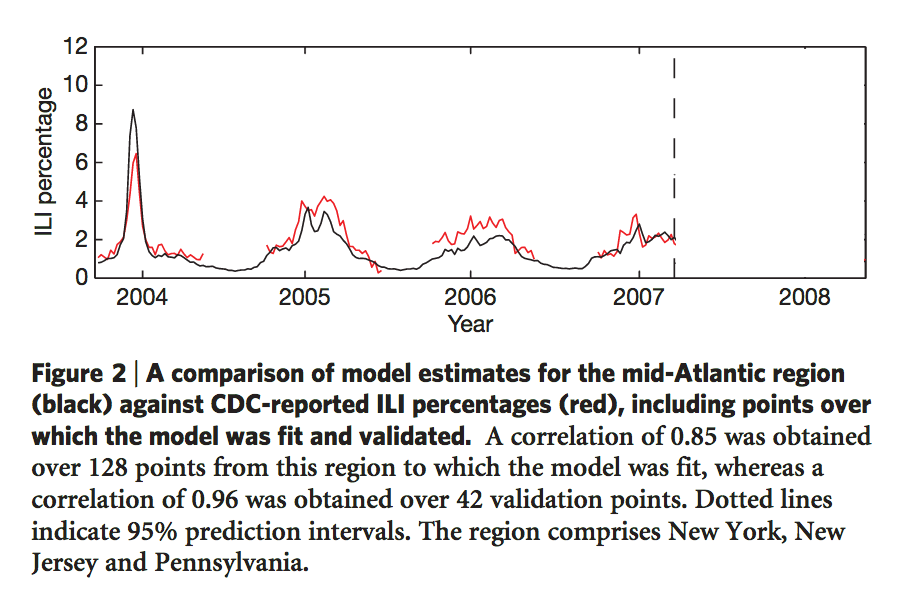
\includegraphics[width=\textwidth]{figures/ginsberg_detecting_2009_fig2_insample}
\end{center}

\end{frame}
%%%%%%%%%%%%%%%%%%%%%%%%%
\begin{frame}

\begin{center}
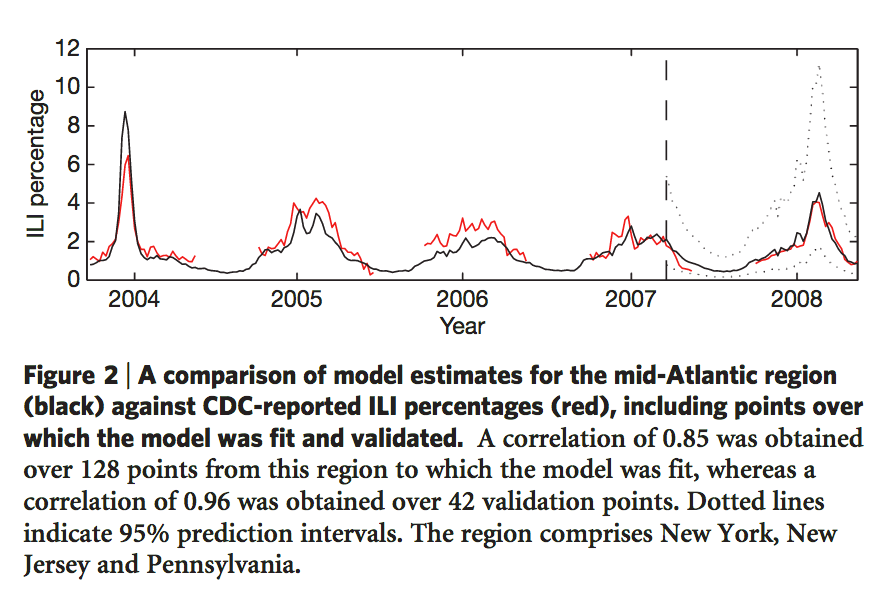
\includegraphics[width=\textwidth]{figures/ginsberg_detecting_2009_fig2}
\end{center}

\end{frame}
%%%%%%%%%%%%%%%%%%%%%%%%%
\begin{frame}

\begin{center}
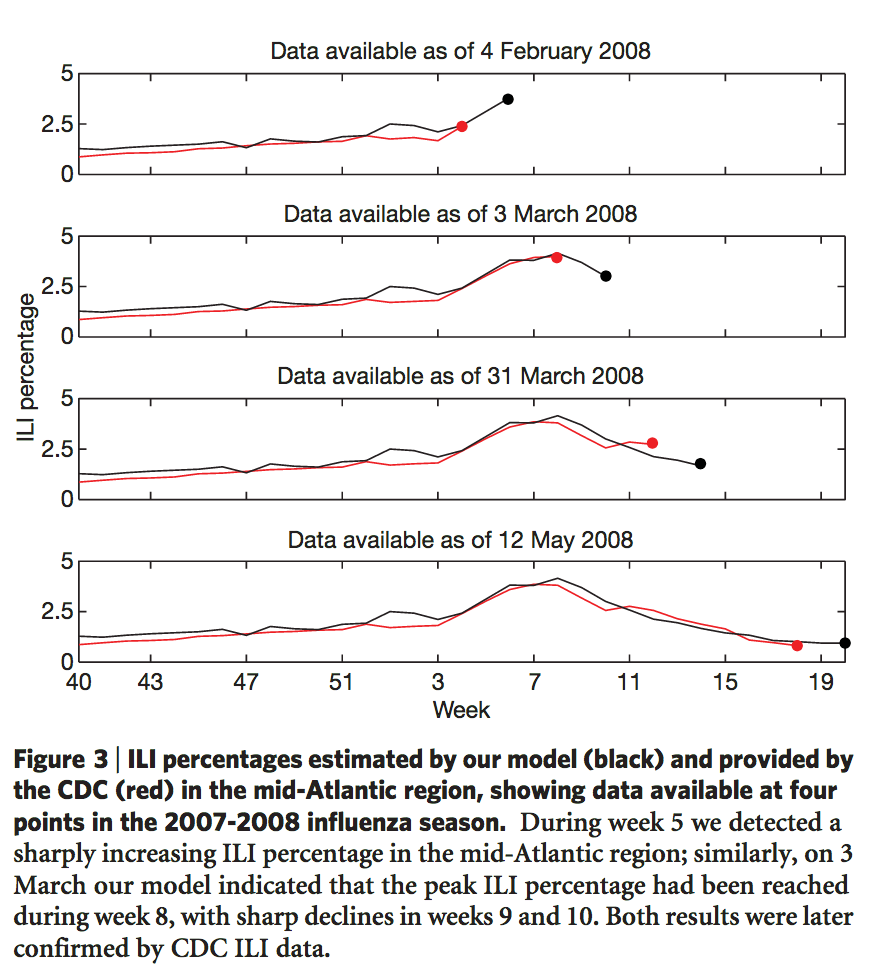
\includegraphics[width=0.6\textwidth]{figures/ginsberg_detecting_2009_fig3}
\end{center}

\end{frame}
%%%%%%%%%%%%%%%%%%%%%%%%%
\begin{frame}

\begin{center}
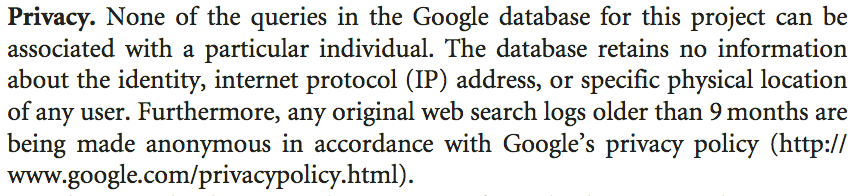
\includegraphics[width=\textwidth]{figures/ginsberg_detecting_2009_privacy}
\end{center}
\pause

\begin{itemize}
\item \textcolor{green}{Make a deontological argument against doing this study without consent.}
\pause
\item \textcolor{green}{Make a consequentialist argument for doing this study without consent.}
\end{itemize}

\end{frame}
%%%%%%%%%%%%%%%%%%%%%%%%%
\begin{frame}

\textcolor{green}{Which do you prefer?}
\begin{enumerate}
\item Researcher selected keywords (Polgreen et al., 2008) 
\item Data selected keywords (Ginsberg et al., 2009)
\end{enumerate}

\end{frame}
%%%%%%%%%%%%%%%%%%%%%%%%%
\begin{frame}

Researchers selected key-words (Polgreen et al., 2008) 
\begin{itemize}
\item takes advantage of researcher knowledge
\item limits risk of over-fitting
\item can be done without enormous amounts of data
\end{itemize}

\pause

Data-driven keyword selection (Ginsberg et al., 2009)
\begin{itemize}
\item generalized to every time-series all over the world
\item potentially discovers surpassingly good predictors (e.g., antibiotic related queries)
\item risks over-fitting 
\item requires lots of data and computing
\end{itemize}

\end{frame}
%%%%%%%%%%%%%%%%%%%%%%%%%
\begin{frame}

\begin{center}
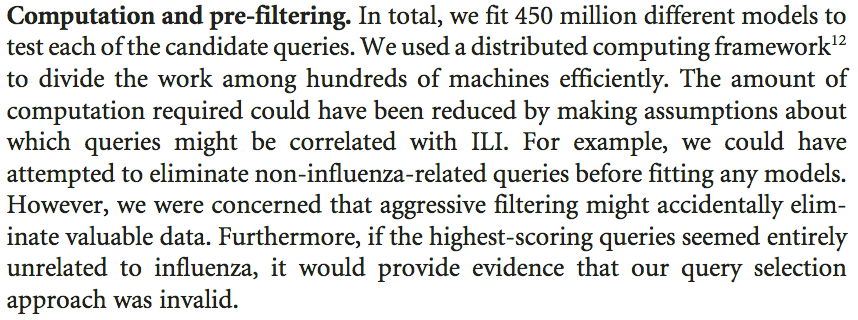
\includegraphics[width=\textwidth]{figures/ginsberg_detecting_2009_filtering}
\end{center}

\end{frame}
%%%%%%%%%%%%%%%%%%%%%%%%%
\begin{frame}

\textcolor{green}{What do you think?}
\begin{enumerate}
\item Game changer
\item Incremental improvement
\end{enumerate}

\end{frame}
%%%%%%%%%%%%%%%%%%%%%%%%%
\begin{frame}

\begin{center}
\begin{tabular}{ccc}
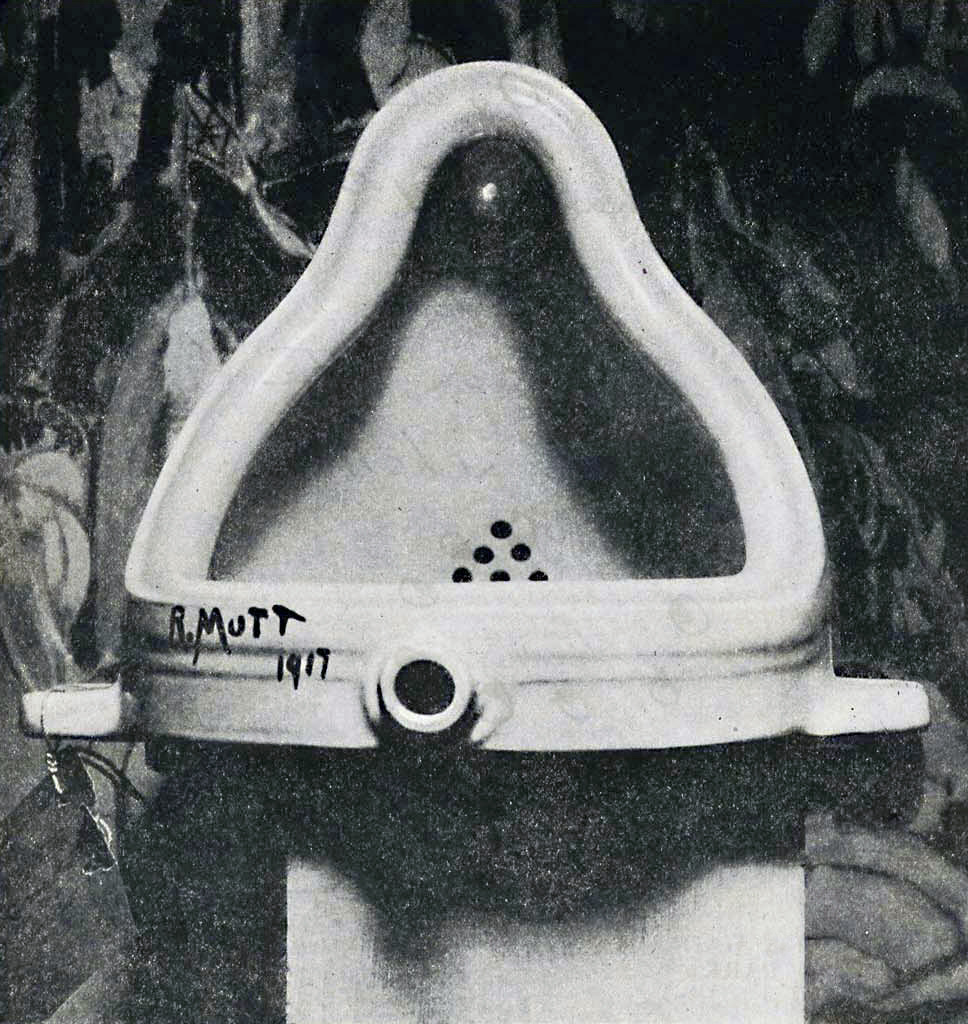
\includegraphics[width=0.30\textwidth]{figures/duchamp_fountain} & \phantom{12345} & 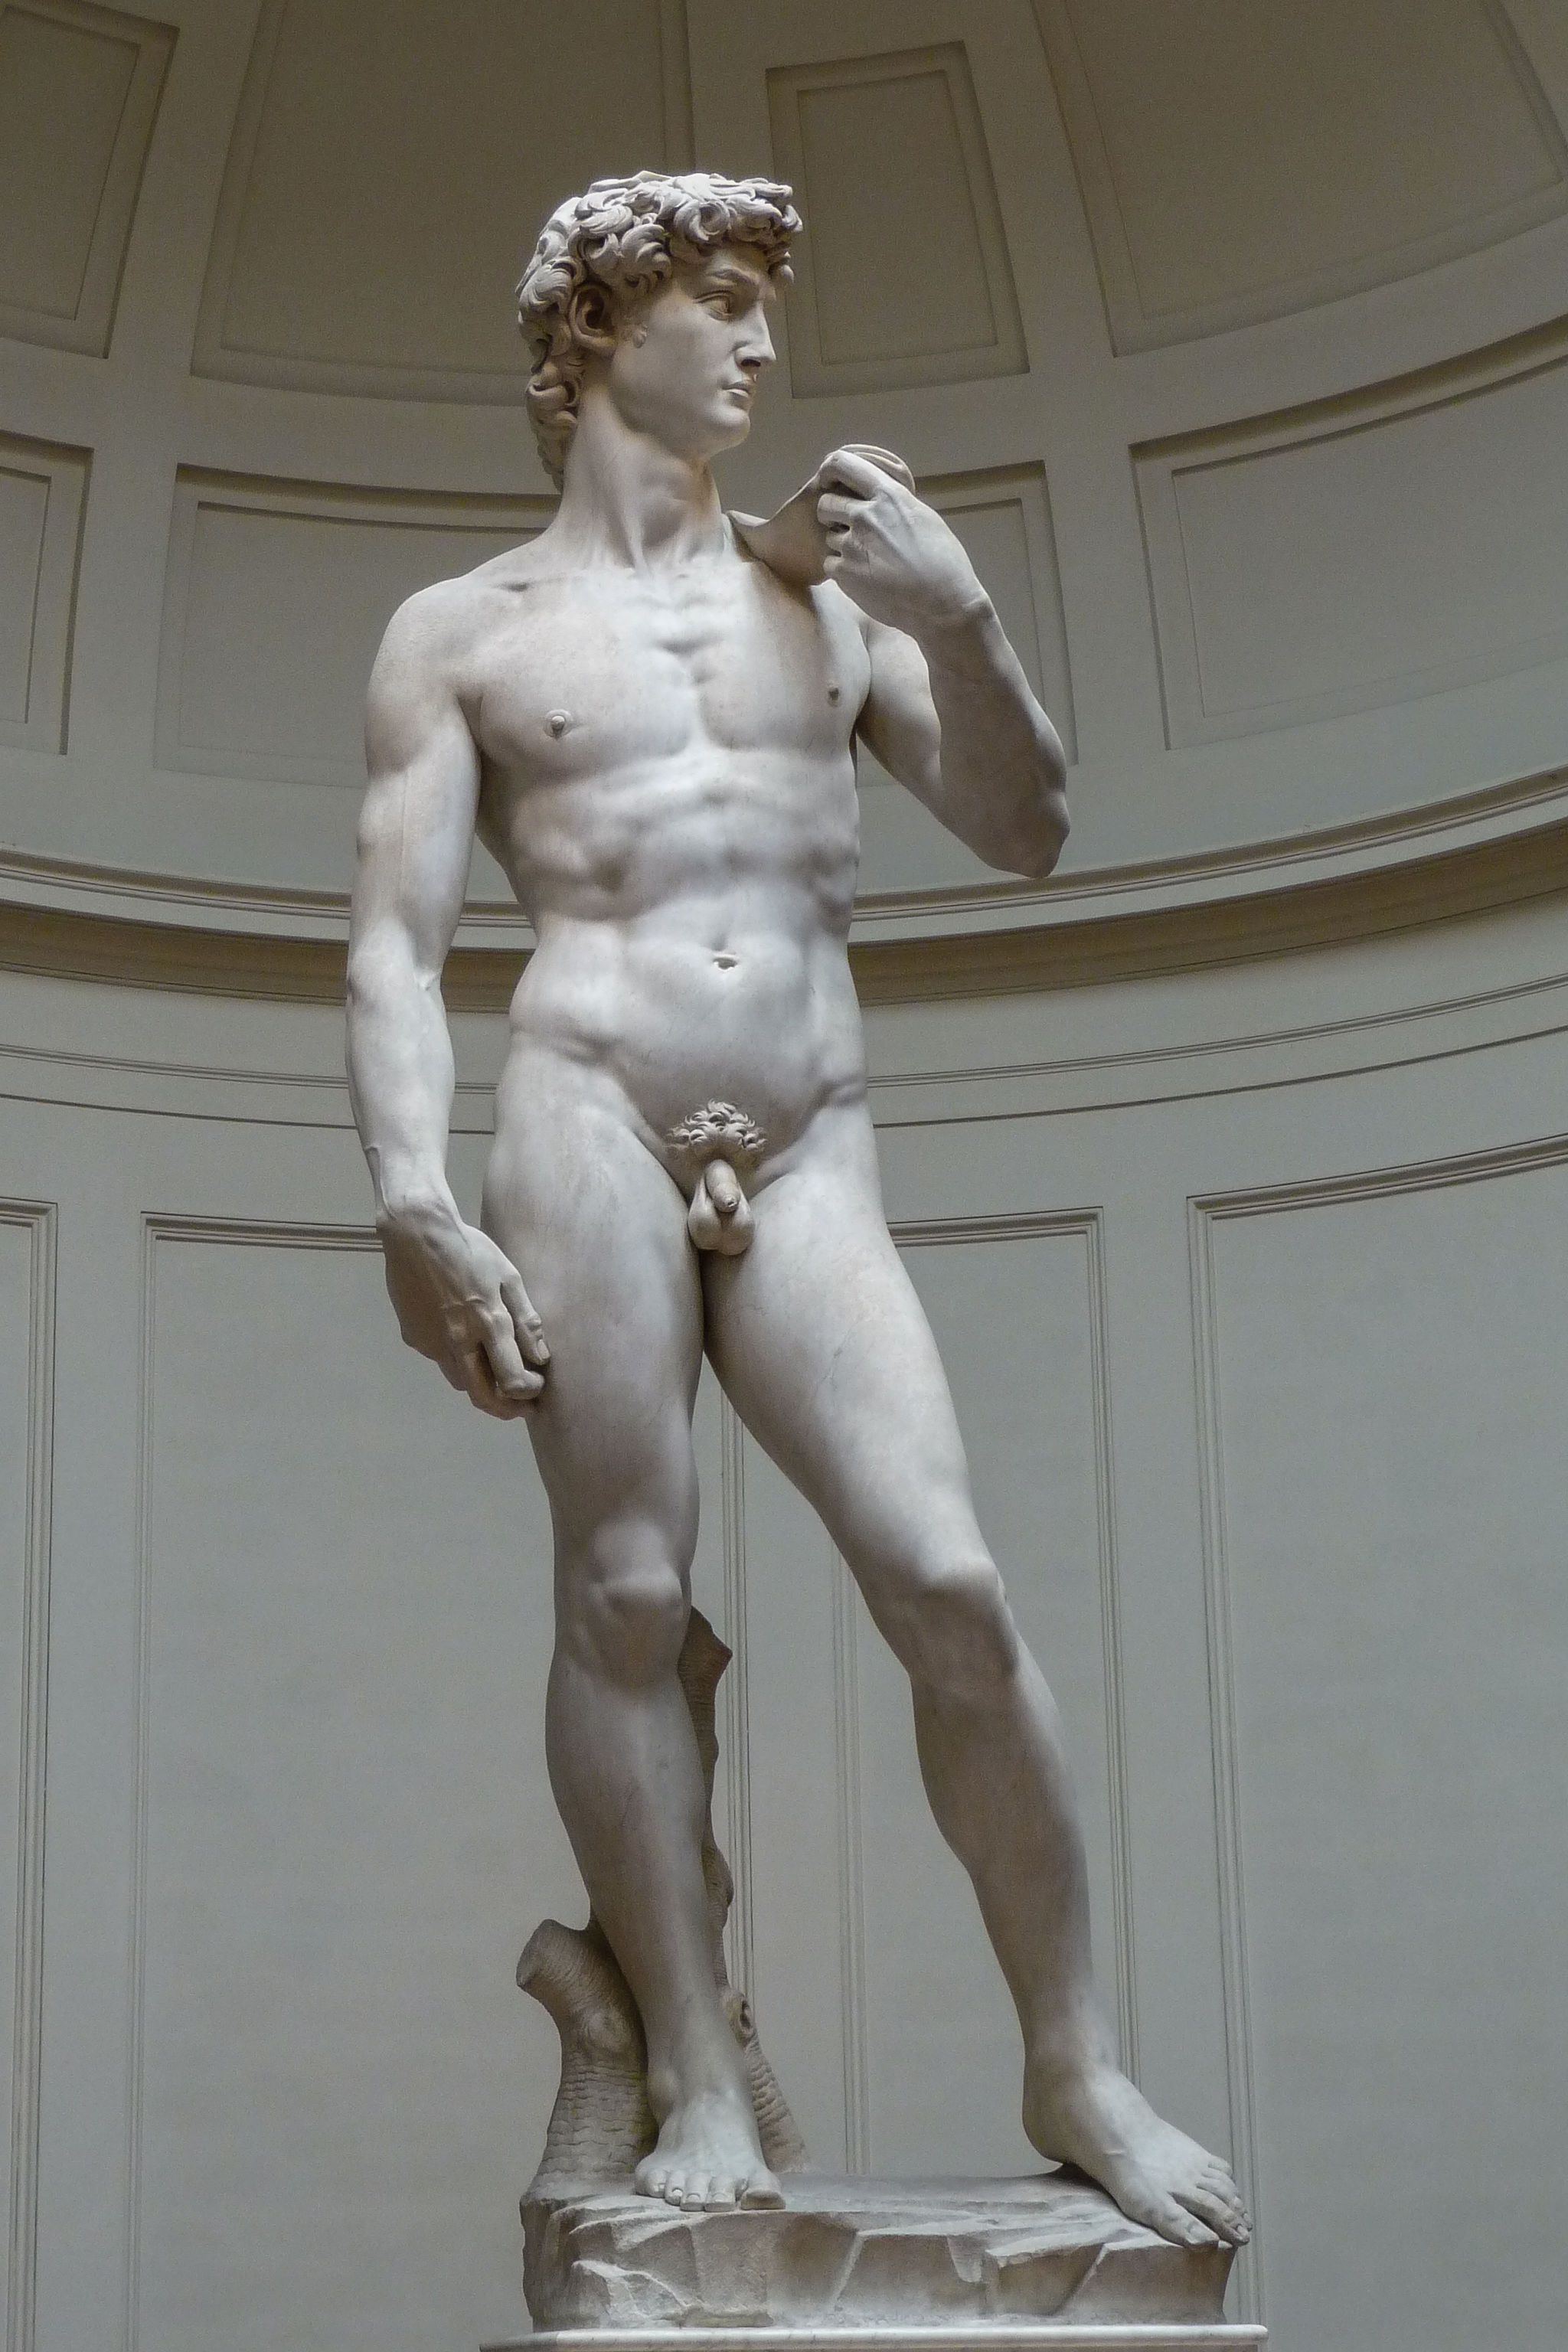
\includegraphics[width=0.30\textwidth]{figures/michelangelo_david} \\
\LARGE{Readymades} &  & \LARGE{Custommades}
\end{tabular}
\end{center}

\vf
\vspace{0.5in}
\TINY{\url{https://commons.wikimedia.org/wiki/File:Duchamp_Fountaine.jpg}}\\
\TINY{\url{https://commons.wikimedia.org/wiki/File:\%27David\%27_by_Michelangelo_JBU0001.JPG}}

\end{frame}
%%%%%%%%%%%%%%%%%%%%%%%s
\begin{frame}

\begin{center}

\includegraphics[width=\textwidth]{figures/goel_predicting_2010_title}
\end{center}

Goel et al 2010.

\end{frame}
%%%%%%%%%%%%%%%%%%%%%%%%%%
\begin{frame}

\begin{center}
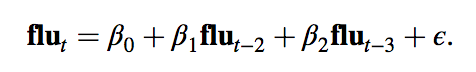
\includegraphics[width=\textwidth]{figures/goel_predicting_2010_flu}
\end{center}

\end{frame}
%%%%%%%%%%%%%%%%%%%%%%%%%%
\begin{frame}

\begin{center}
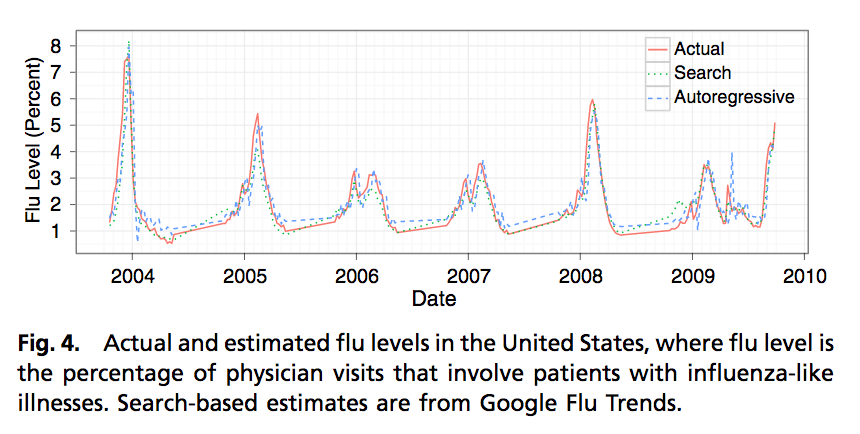
\includegraphics[width=\textwidth]{figures/goel_predicting_2010_fig4}
\end{center}

\end{frame}
%%%%%%%%%%%%%%%%%%%%%%%%%%
\begin{frame}

{\Large
\begin{center}
Did this change how you think about Ginsberg et al 2009?
\end{center}
}

\end{frame}
%%%%%%%%%%%%%%%%%%%%%%%%%%
\begin{frame}

Can search predict revenue?
\begin{center}
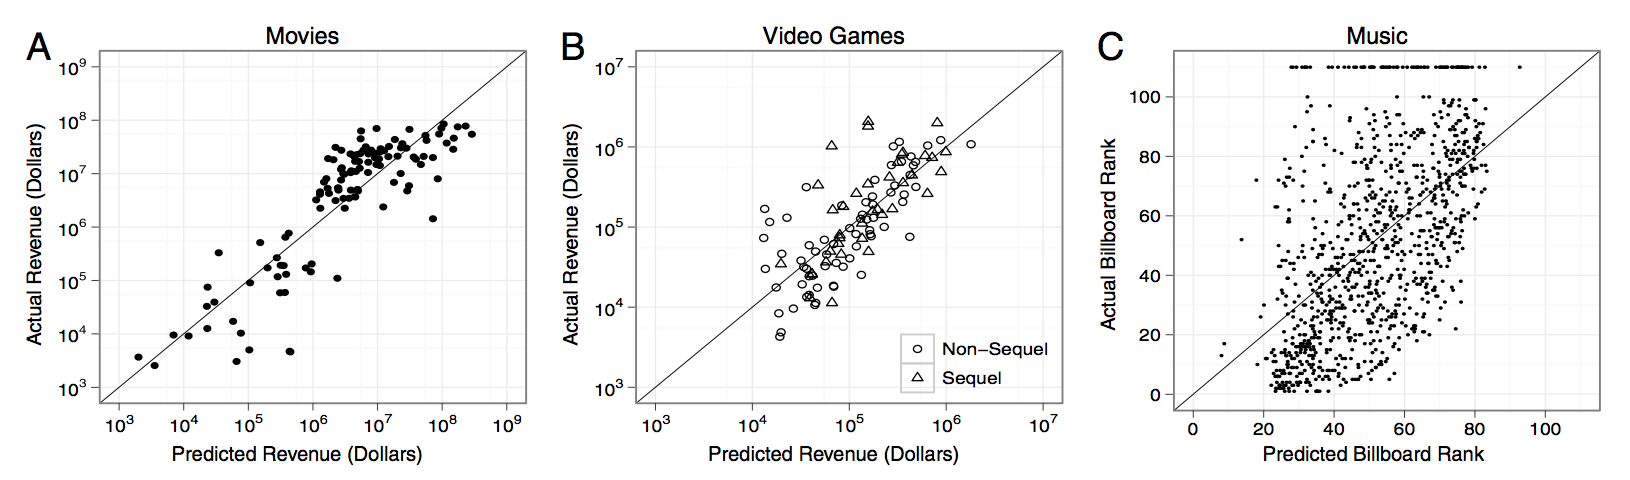
\includegraphics[width=\textwidth]{figures/goel_predicting_2010_fig2a-c}
\end{center}
\vf
Wrong question

\end{frame}
%%%%%%%%%%%%%%%%%%%%%%%%%%
\begin{frame}

How much can search improve simple baseline prediction?
\begin{center}
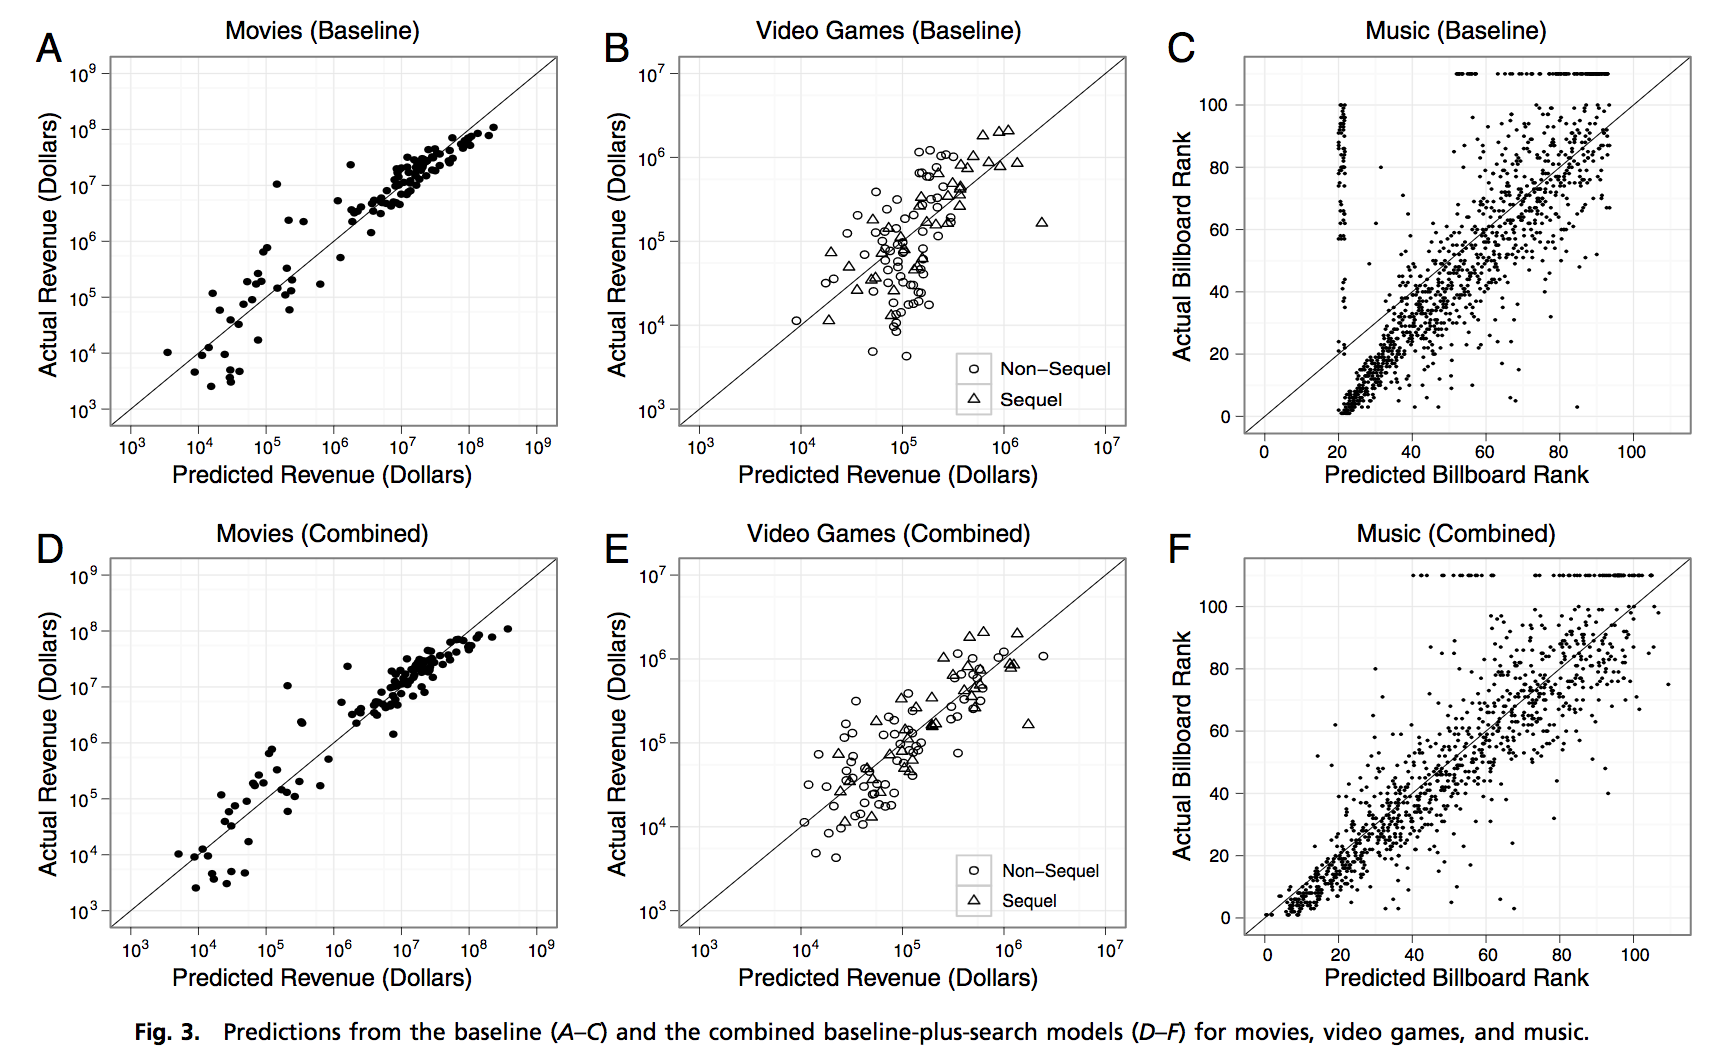
\includegraphics[width=\textwidth]{figures/goel_predicting_2010_fig3}
\end{center}
\vf
Right question

\end{frame}
%%%%%%%%%%%%%%%%%%%%%%%%%%
\begin{frame}

\begin{center}
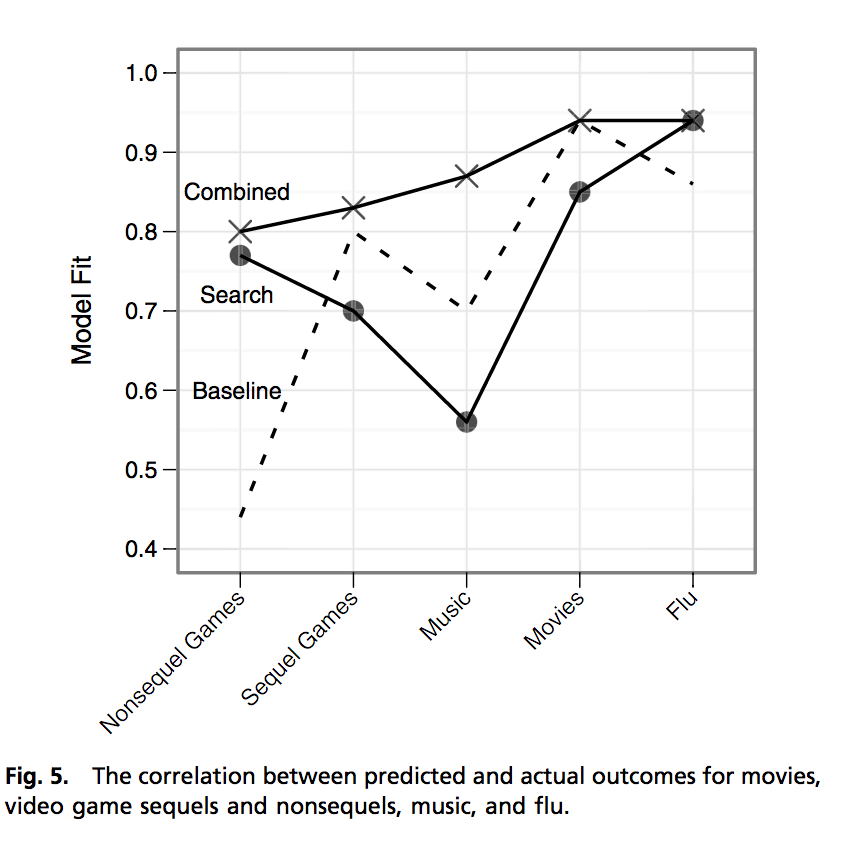
\includegraphics[width=\textwidth]{figures/goel_predicting_2010_fig5}
\end{center}

\end{frame}
%%%%%%%%%%%%%%%%%%%%%%%%%%
\begin{frame}

Key idea from data science:\\
Predictions have to be compared to something else\\
\pause
Tamara: the app you mentioned

\end{frame}
%%%%%%%%%%%%%%%%%%%%%%%%%%
\begin{frame}

{\Large
\begin{center}
Aside: See how the figures tell the story of this paper.
\end{center}
}

\end{frame}
%%%%%%%%%%%%%%%%%%%%%%%%%%
\begin{frame}

\begin{center}

\includegraphics[width=\textwidth]{figures/cook_assessing_2011_title}
\end{center}

\vf

Cook et al. (2011) ``Assessing Google Flu Trends Performance in the United States during the 2009 Influenza Virus A (H1N1) Pandemic.'' \textit{PLoS ONE}, \url{http://dx.doi.org/10.1371/journal.pone.0023610}

\end{frame}
%%%%%%%%%%%%%%%%%%%%%%%%%%
\begin{frame}

\begin{center}
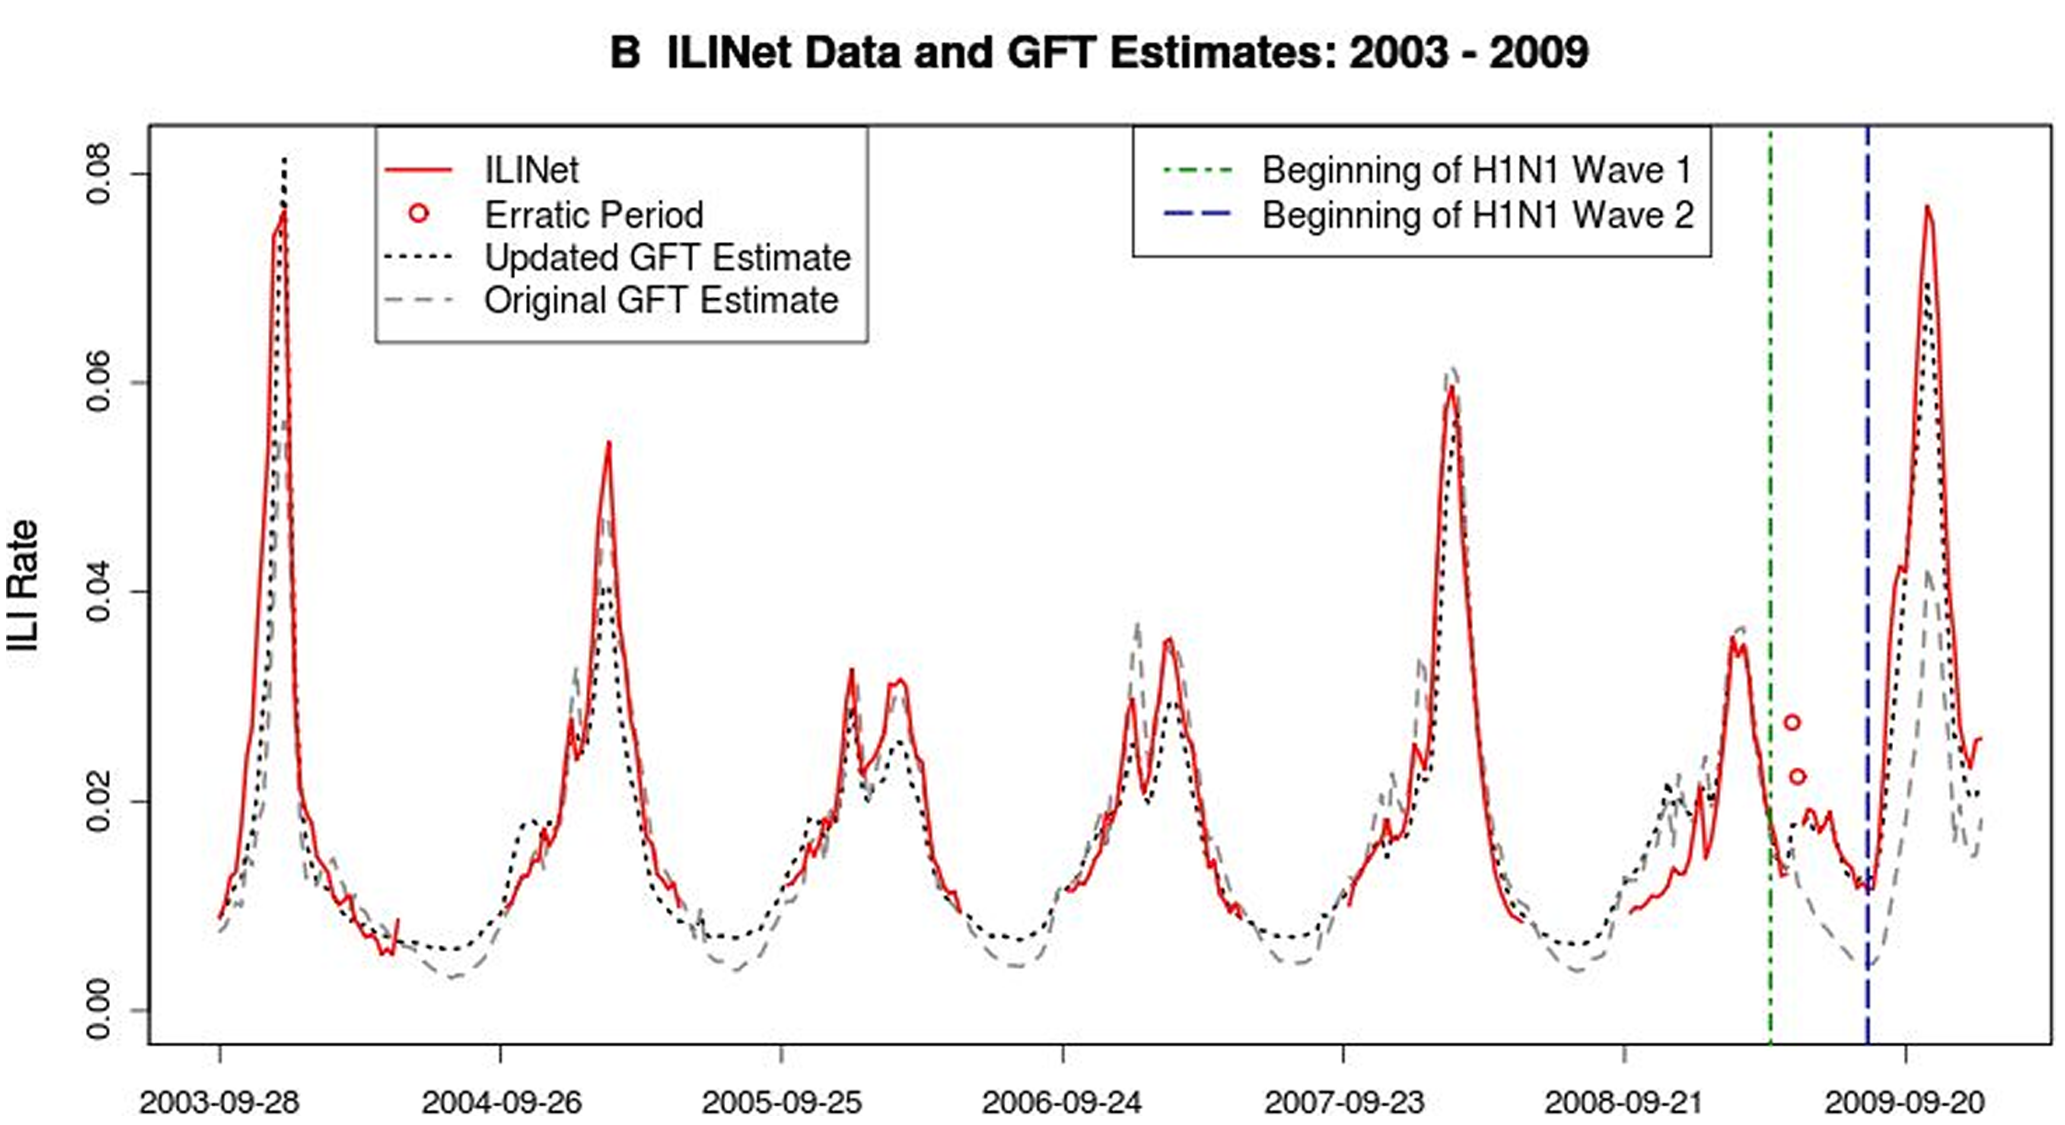
\includegraphics[width=\textwidth]{figures/cook_assessing_2011_fig2b}
\end{center}

\end{frame}
%%%%%%%%%%%%%%%%%%%%%%%%%%
\begin{frame}

\begin{center}
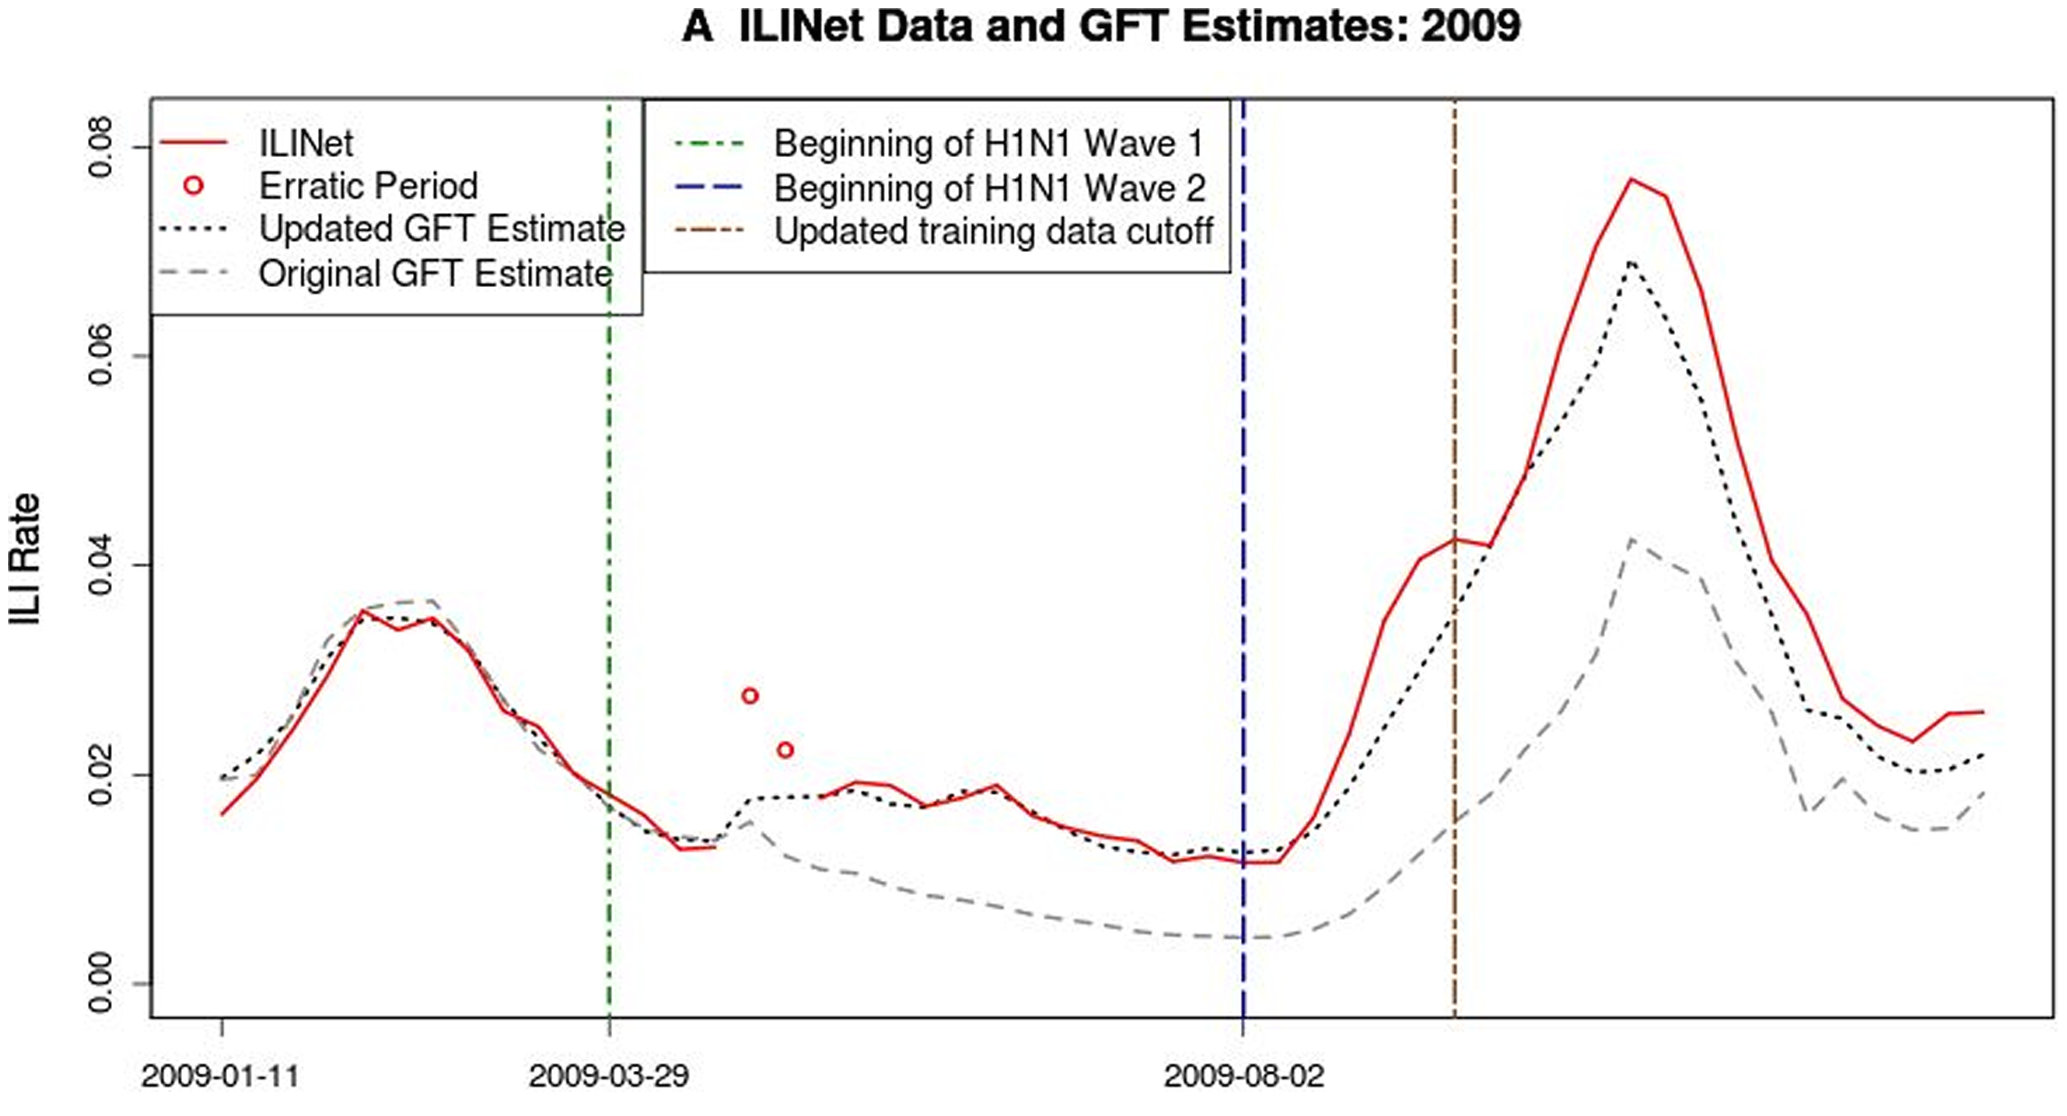
\includegraphics[width=\textwidth]{figures/cook_assessing_2011_fig2a}
\end{center}

\end{frame}
%%%%%%%%%%%%%%%%%%%%%%%%%%
\begin{frame}

\begin{center}
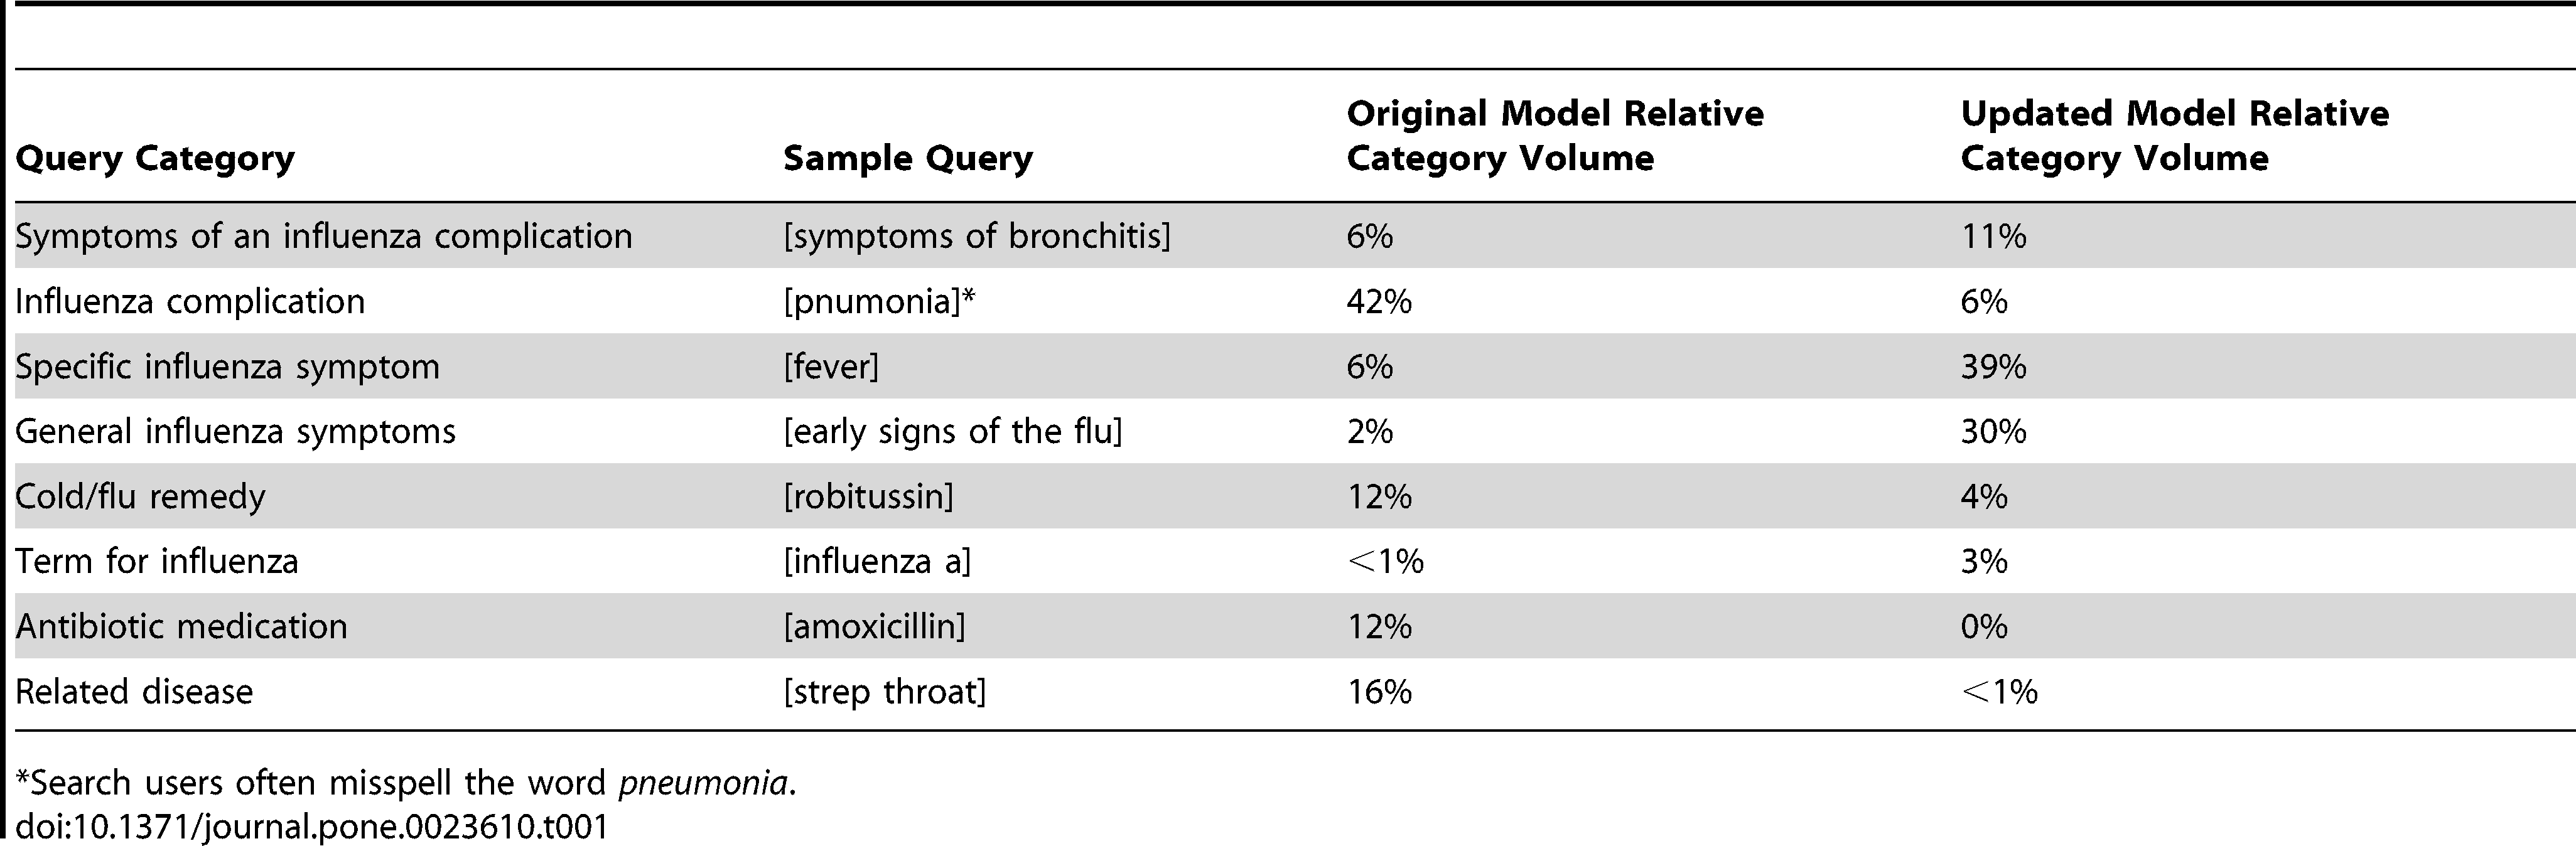
\includegraphics[width=\textwidth]{figures/cook_assessing_2011_tab1}
\end{center}

\end{frame}
%%%%%%%%%%%%%%%%%%%%%%%%%%
\begin{frame}

\begin{center}
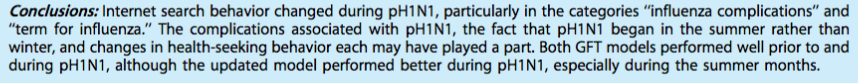
\includegraphics[width=\textwidth]{figures/cook_assessing_2011_conclusion}
\end{center}

\end{frame}
%%%%%%%%%%%%%%%%%%%%%%%%%%
\begin{frame}

\begin{center}
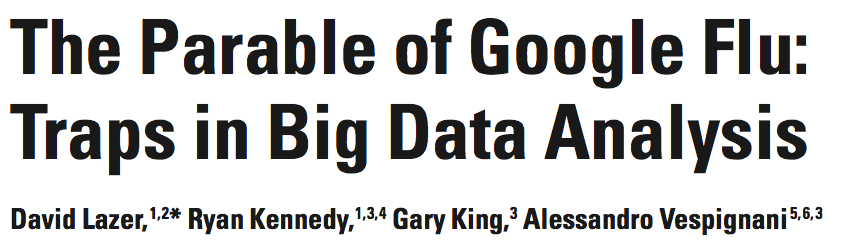
\includegraphics[width=\textwidth]{figures/lazer_parable_2014_title}
\end{center}

\vf 
Lazer et al (2014) ``The Parable of Google Flu: Traps in Big Data Analysis.'' \textit{Science}. \url{http://dx.doi.org/10.1126/science.1248506}

\end{frame}
%%%%%%%%%%%%%%%%%%%%%%%%%%
\begin{frame}

\begin{center}
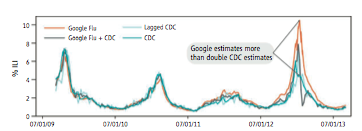
\includegraphics[width=\textwidth]{figures/lazer_parable_2014_fig1a}
\end{center}

\end{frame}
%%%%%%%%%%%%%%%%%%%%%%%%%%
\begin{frame}

\begin{center}
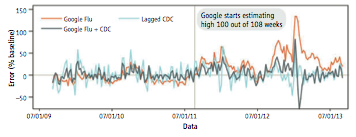
\includegraphics[width=\textwidth]{figures/lazer_parable_2014_fig1b}
\end{center}

\end{frame}
%%%%%%%%%%%%%%%%%%%%%%%%%%
\begin{frame}

\textcolor{green}{What are the differences between these plots?}

\begin{center}
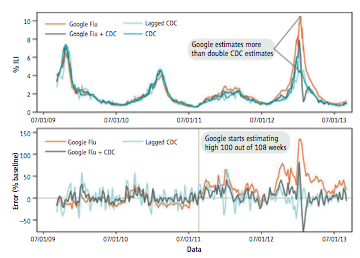
\includegraphics[width=\textwidth]{figures/lazer_parable_2014_fig1}
\end{center}

\end{frame}
%%%%%%%%%%%%%%%%%%%%%%%%%%
\begin{frame}

\begin{itemize}
\item Big data hubris\\
Basically not paying attention
\pause
\item Algorithm dynamics (combines what I called algorithmic confounding and drift)\\
Adding recommended searches to increase health related queries
\end{itemize}

\end{frame}
%%%%%%%%%%%%%%%%%%%%%%%%%%
\begin{frame}

\begin{itemize}
\item Big data hubris\\
Basically not paying attention
\pause
\item Algorithm dynamics (combines what I called algorithmic confounding and drift)\\
Adding recommended searches to increase health related queries
\end{itemize}

\end{frame}
%%%%%%%%%%%%%%%%%%%%%%%%%%
\begin{frame}

Projecting from the past to the present only works if nothing in the world changes; there is no model, no mechanism for understanding; this is blind curve-fitting

\end{frame}
%%%%%%%%%%%%%%%%%%%%%%%%%%
\begin{frame}

\begin{itemize}
\item Transparency and replicability
\pause
\textcolor{green}{What do you think Google should do in this case?}
\item Using big data to understand the unknown (basically estimate quantities that can't be estimated otherwise)
\pause
\item Study the algorithm (Malte and Arvind)
\pause
\item It's not just about size of the data (calls for a hybrid between ``big'' and ``small'' data researchers)
\end{itemize}

\end{frame}
%%%%%%%%%%%%%%%%%%%%%%%%%%
\begin{frame}

Aside: note how this more general framing improves impact of paper

\end{frame}
%%%%%%%%%%%%%%%%%%%%%%%%%%
\begin{frame}

\begin{center}
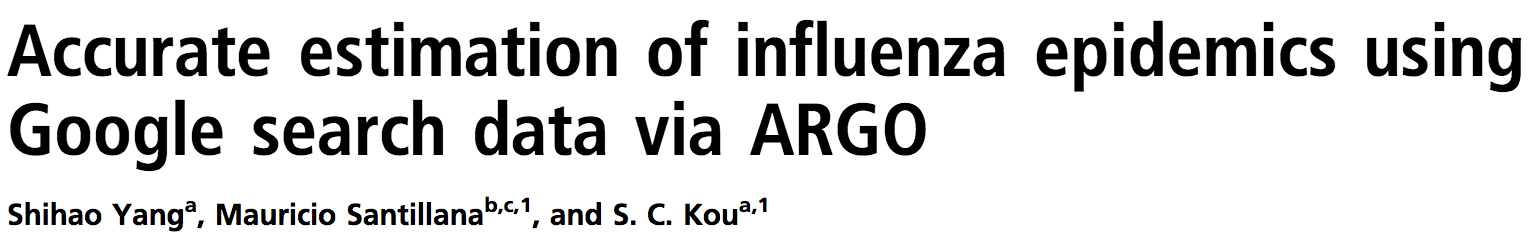
\includegraphics[width=\textwidth]{figures/yang_accurate_2015_title}
\end{center}

\vf
Yang et al (2015) ``Accurate estimation of influenza epidemics using Google search data via ARGO'', \textit{PNAS}, \url{http://dx.doi.org/10.1073/pnas.1515373112}
\end{frame}
%%%%%%%%%%%%%%%%%%%%%%%%%%
\begin{frame}

\begin{center}
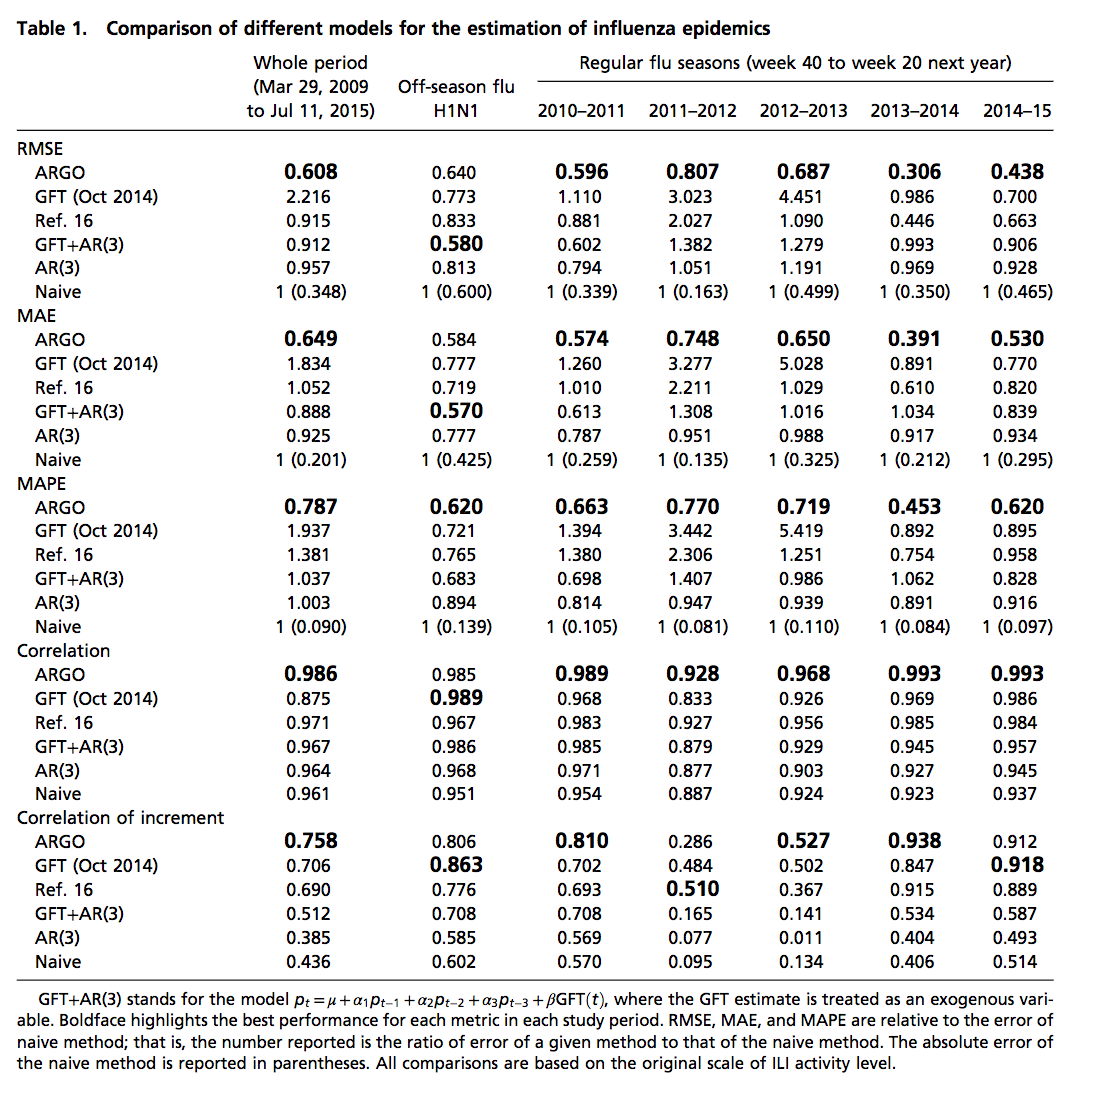
\includegraphics[width=\textwidth]{figures/yang_accurate_2015_tab1}
\end{center}

Note the clear comparison against other methods by clear metrics

\end{frame}
%%%%%%%%%%%%%%%%%%%%%%%%%%
\begin{frame}

\begin{center}
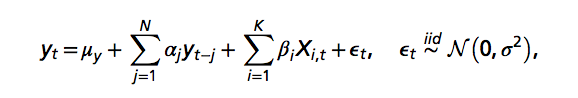
\includegraphics[width=\textwidth]{figures/yang_accurate_2015_eq2}
\end{center}

Combines:
\begin{itemize}
\item lots of lags (statistical issue or fundamental model?)
\item lots of search terms
\item regularization (different way of dealing with over-fitting)
\end{itemize}

\end{frame}
%%%%%%%%%%%%%%%%%%%%%%%%%%
\begin{frame}

\begin{center}
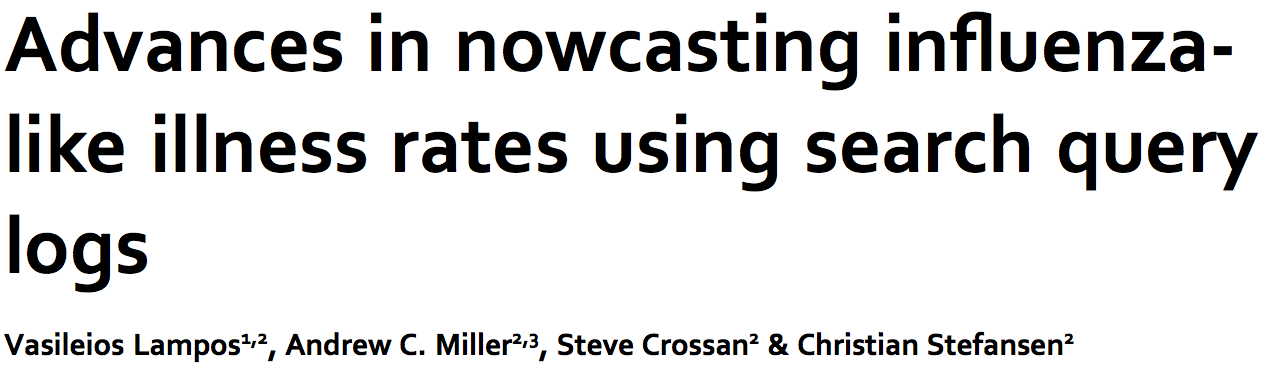
\includegraphics[width=\textwidth]{figures/lampos_advances_2015_title}
\end{center}

Lampos et al 2015 ``Advances in nowcasting influenza-like illness rates using search query logs'' \textit{Scientific Reports}, \url{http://dx.doi.org/10.1038/srep12760}

\end{frame}
%%%%%%%%%%%%%%%%%%%%%%%%%%
\begin{frame}

\begin{itemize}
\item Eysenbach (2006)
\item Polgreen et al (2008)
\item Ginsberg et al (2009)
\item Goel et al (2010)
\item Cook et al (2011)
\item Lazer et al (2014)
\item Yang et al (2015), Lampos et al (2015)
\end{itemize}

\end{frame}
%%%%%%%%%%%%%%%%%%%%%%%%%%
\begin{frame}

{\Large
\begin{center}
Can you think of an area in your field that has made this much progress?
\end{center}
}

\end{frame}
%%%%%%%%%%%%%%%%%%%%%%%%%%

\end{document}
